 \documentclass[a4paper,11pt]{article}

\usepackage[english]{babel}
\usepackage{mathrsfs, amssymb, amsmath, amsthm, enumerate}
\usepackage{verbatim, graphicx, geometry, color}
%\usetikzlibrary{arrows}
\usepackage[utf8]{inputenc}
\usepackage{authblk}
\usepackage[round]{natbib}
\bibliographystyle{plainnat}
\usepackage{hyperref}

\makeatletter
\def\@biblabel#1{\hspace*{-\labelsep}}
\makeatother
\geometry{left=1in,right=1
in,top=1.2in,bottom=1.5in}
\newdimen\dummy
\dummy=\oddsidemargin
\addtolength{\dummy}{72pt}
\marginparwidth=.5\dummy
\marginparsep=.1\dummy

\theoremstyle{prop}
\newtheorem{prop}{Proposition}
\theoremstyle{lemma}
\newtheorem{lemma}{Lemma}

\newcommand{\E}{\mathbb{E}}
\newcommand{\Var}{\mathrm{Var}}
\newcommand{\plim}{\overset{p}{\longrightarrow}}
\newcommand{\dlim}{\overset{d}{\longrightarrow}}

\begin{document}
\title{The Mechanics of Endogenous Innovation and Growth: Evidence from Historical U.S. Patents \\
Quantitative Results}
\author{Alexandre B. Sollaci}
\affil{The University of Chicago}
\date{May 2016}
\maketitle

\section*{25\% subsidy on new technologies for 50 years}

\begin{table}[h!]
\begin{tabular}{|l|l|l|l|}
\hline
&\textbf{No Subsidy}&\textbf{Subsidy}&\textbf{\% Change}\\\hline
\textbf{Welfare}&-0.00010682&-0.00010651&0.0029081\\\hline
\textbf{\# technologies}&65084&79188&0.2167\\\hline
\textbf{Average GDP growth}&0.021318&0.021767&0.021077\\\hline
\end{tabular}

\end{table}

\begin{figure}[h!]
\centering
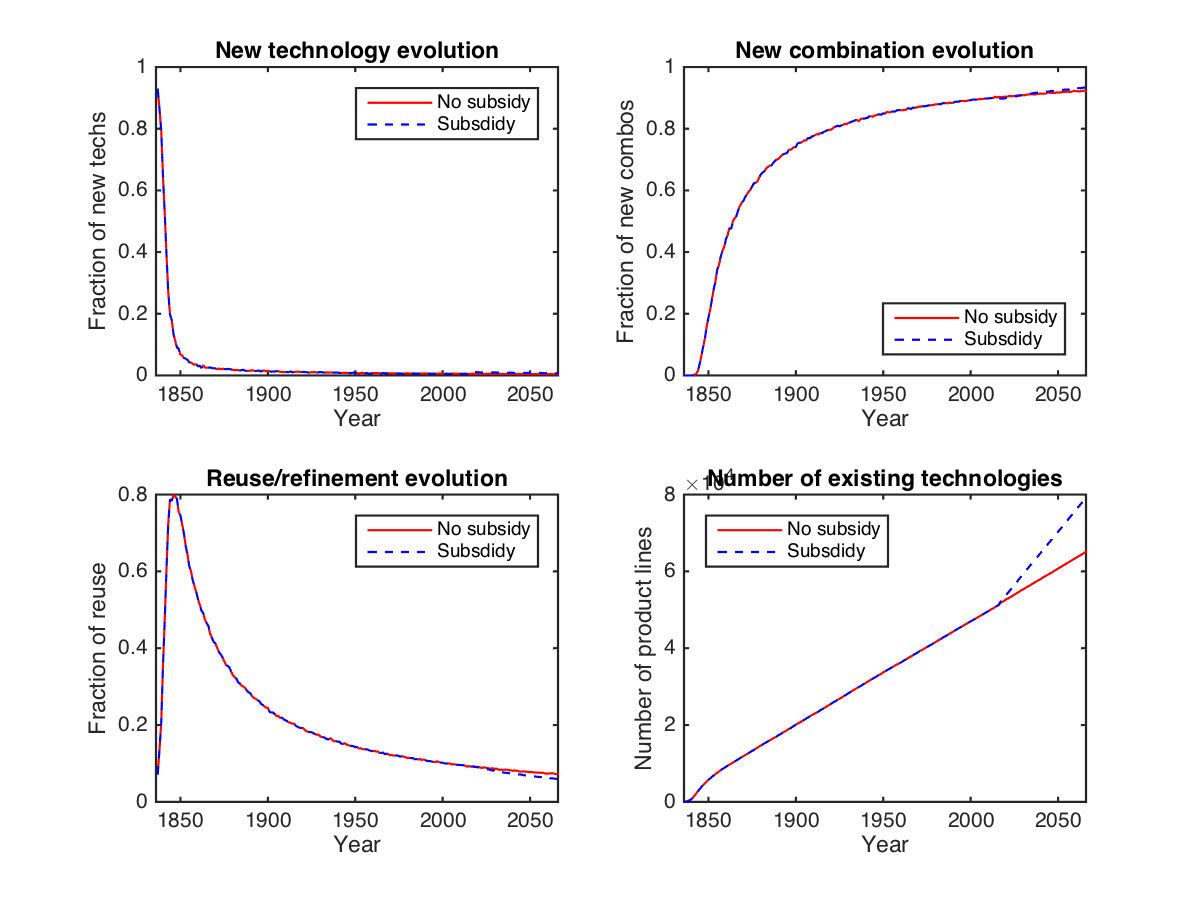
\includegraphics[scale=.6]{patentsNT_50y}
\caption{Evolution of patent shares across the whole period}
\end{figure}

\begin{figure}
\centering
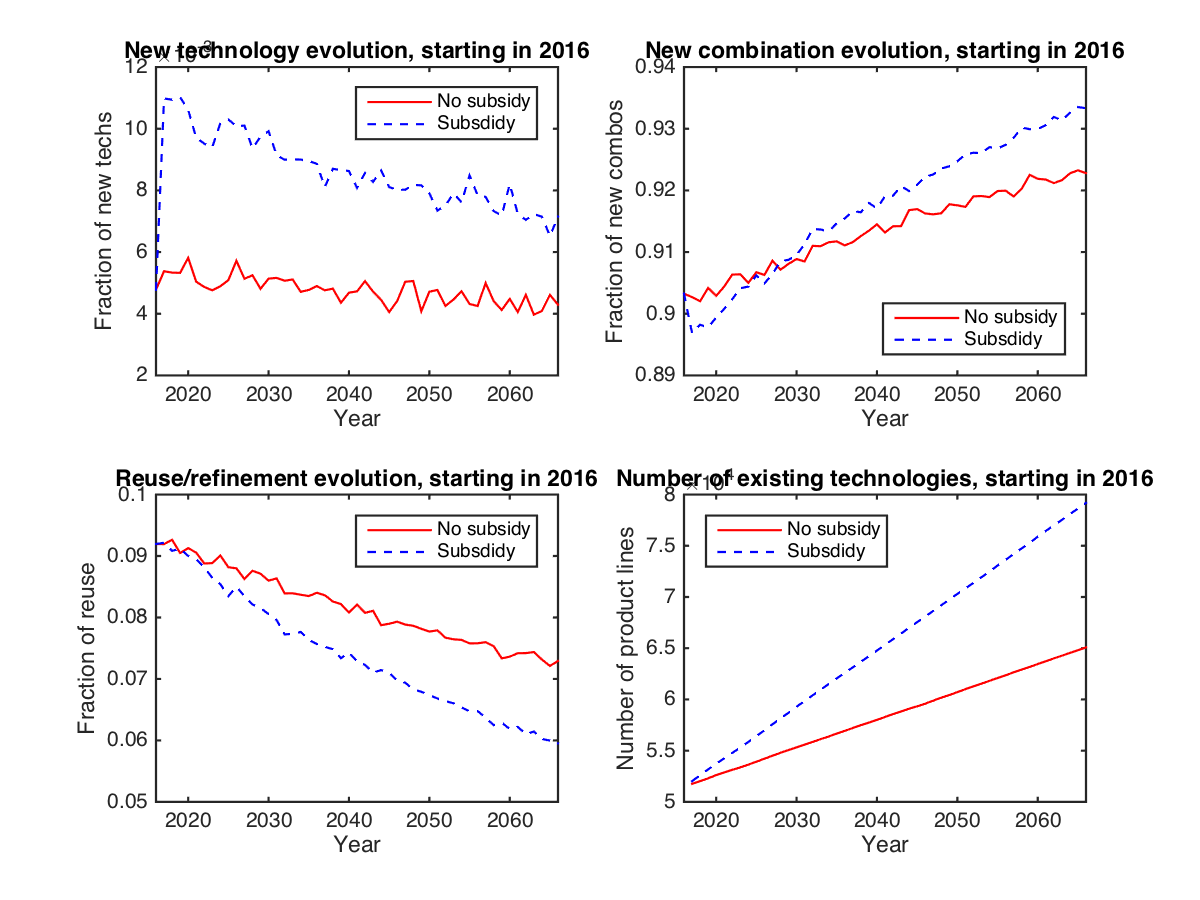
\includegraphics[scale=.6]{patents2016NT_50y}
\caption{Evolution of patent shares, starting in 2016}
\end{figure}

\begin{figure}
\centering
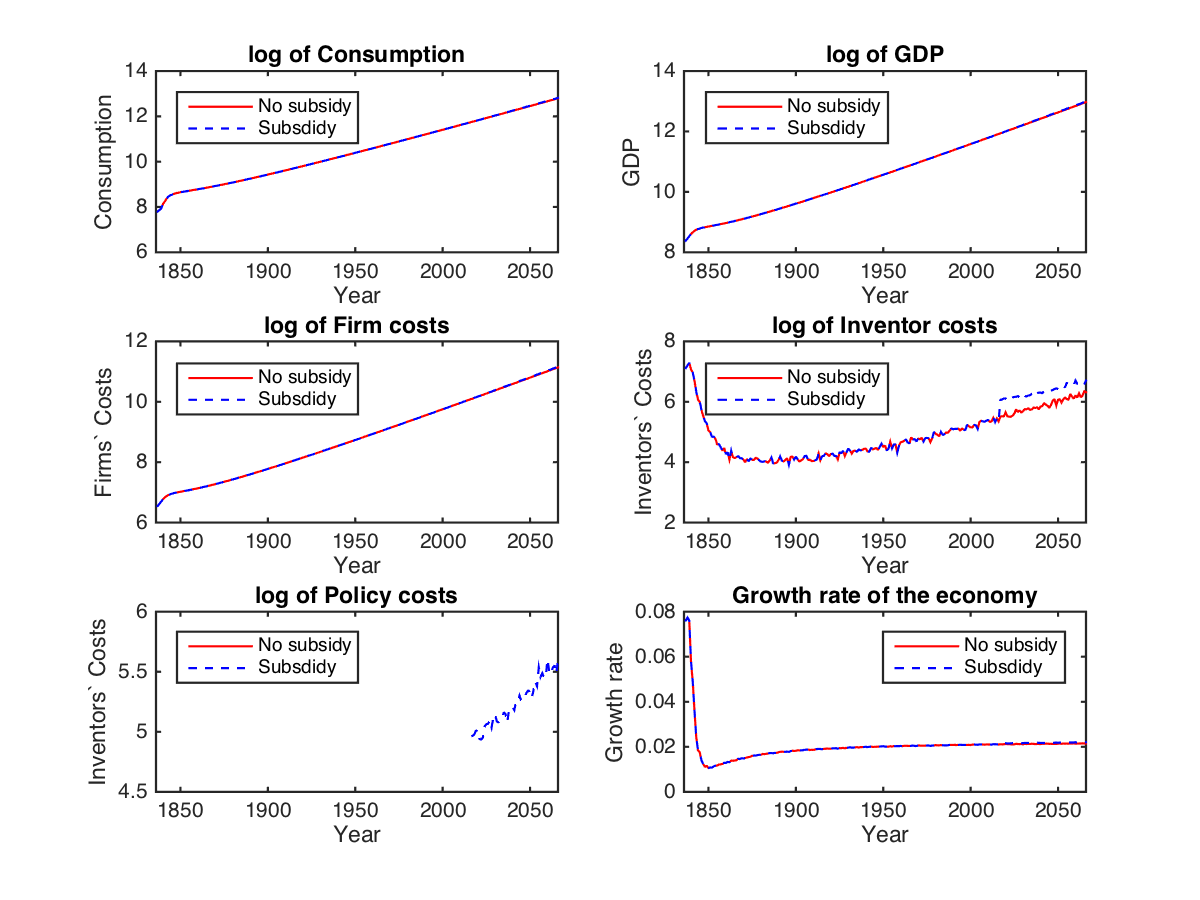
\includegraphics[scale=.6]{aggregatesNT_50y}
\caption{Evolution of aggregate variables over the whole period}
\end{figure}

\begin{figure}
\centering
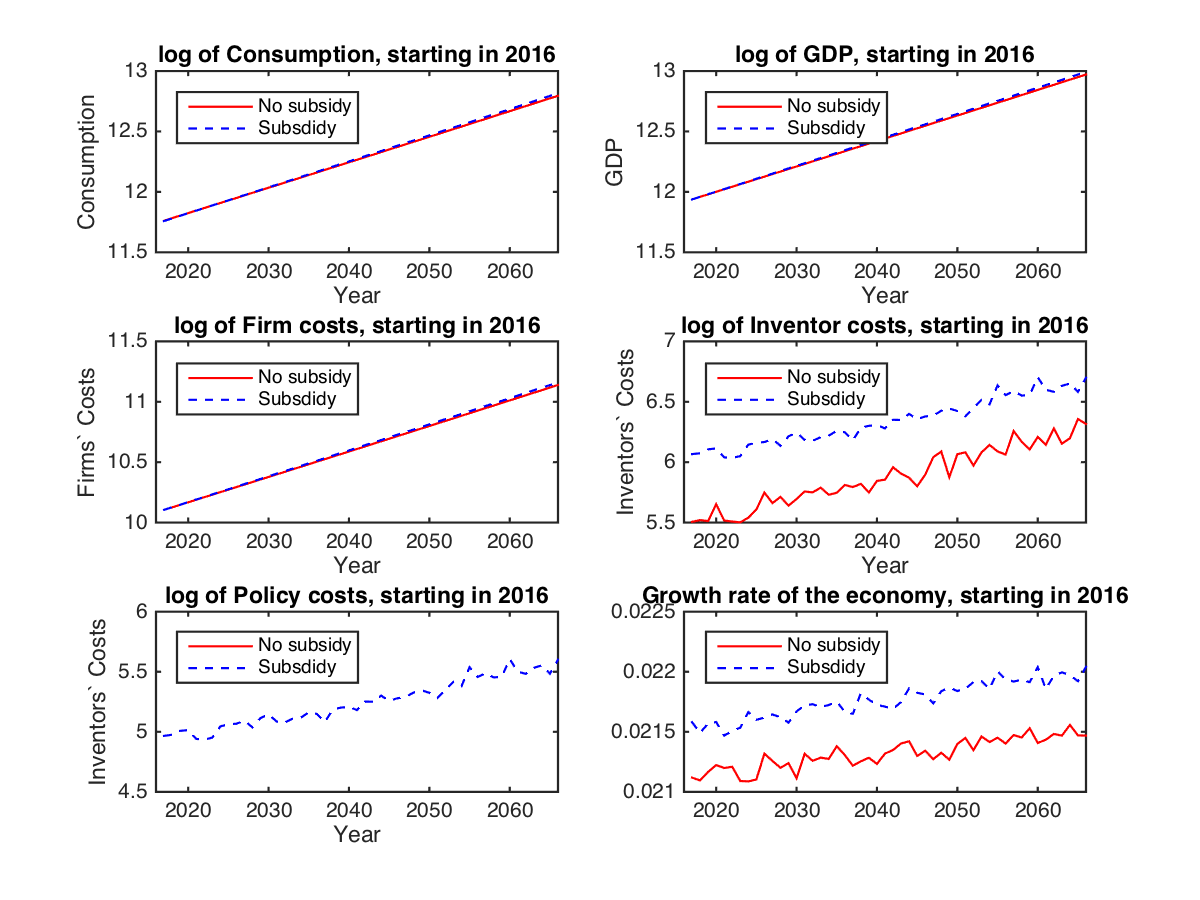
\includegraphics[scale=.6]{aggregates2016NT_50y}
\caption{Evolution of aggregate variables starting in 2016}
\end{figure}

\begin{figure}
\centering
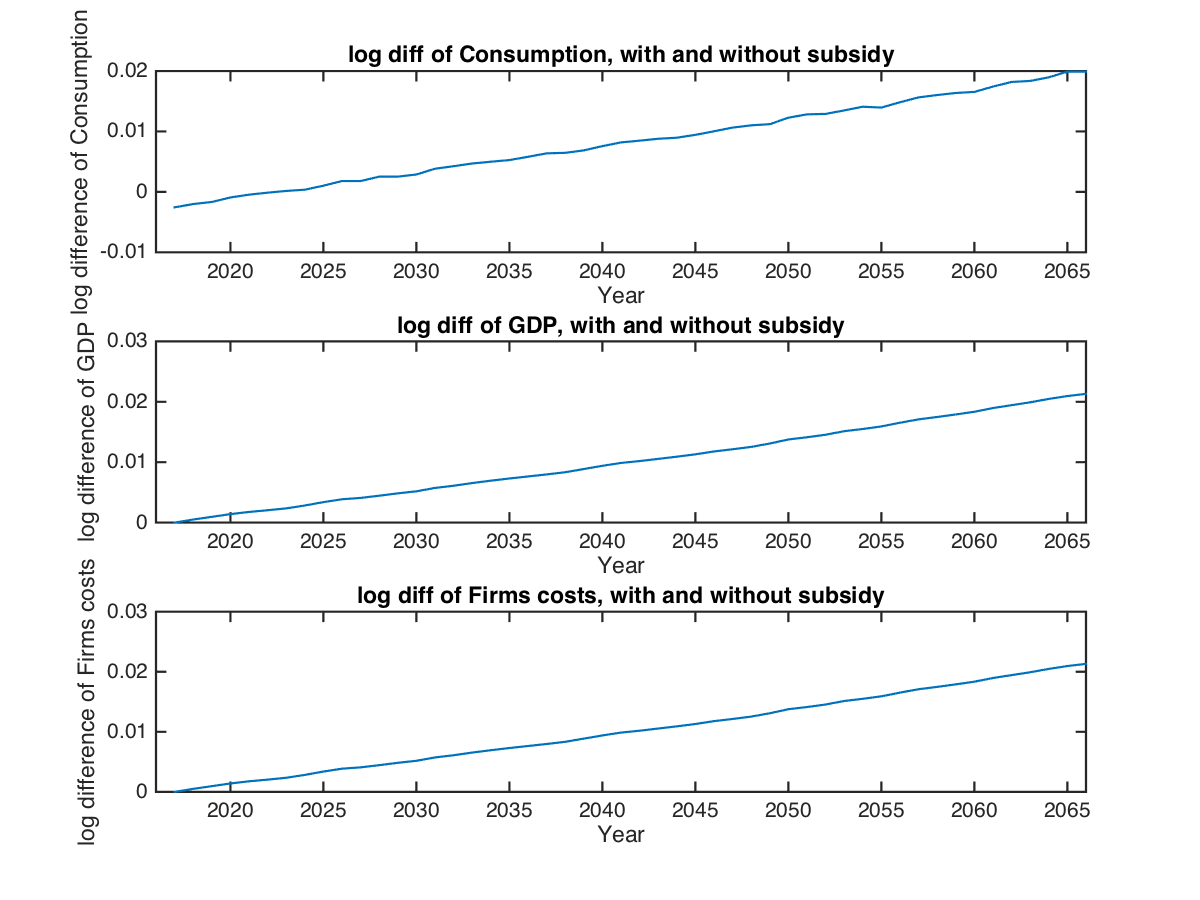
\includegraphics[scale=.6]{aggregates_diffNT_50y}
\caption{Log difference of variables, with subsidy - without subsidy, starting in 2016.}
\end{figure}

\begin{figure}
\centering
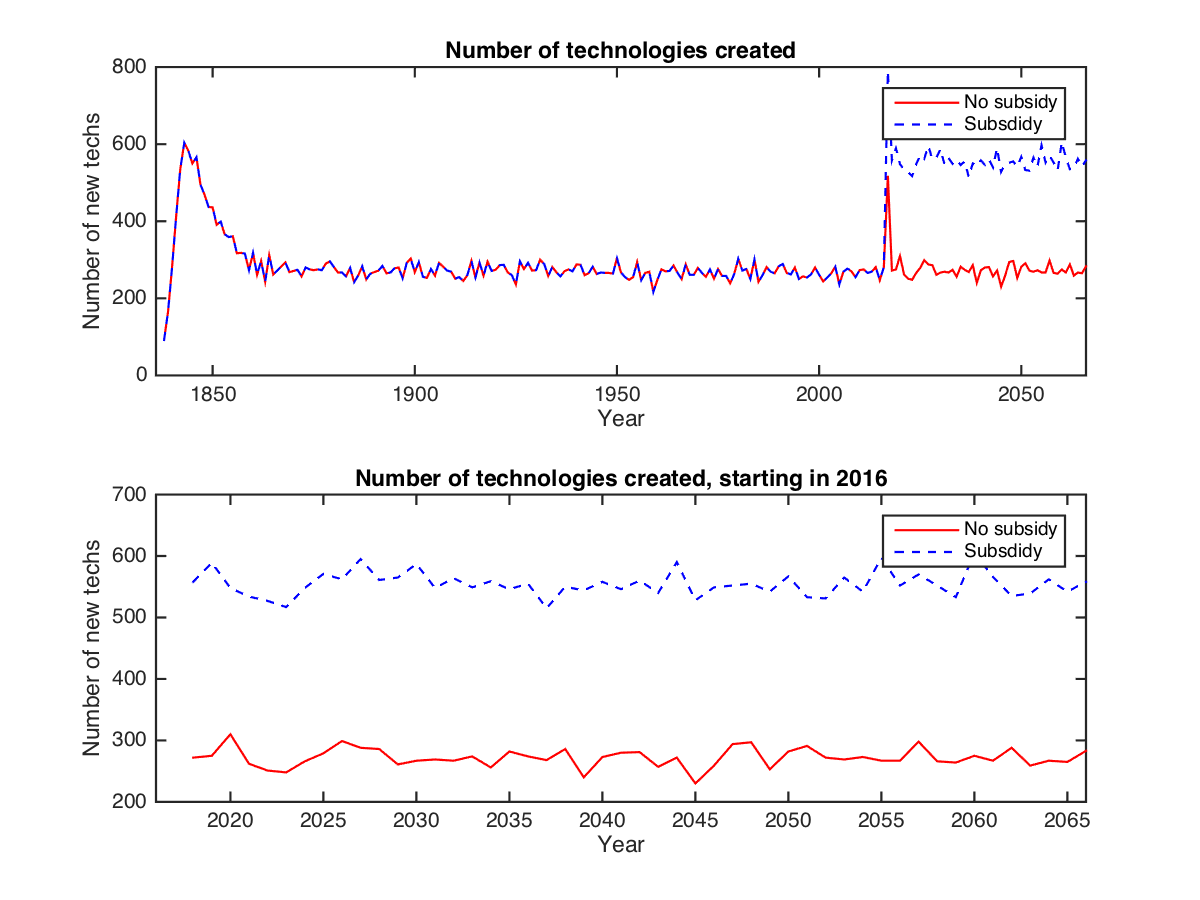
\includegraphics[scale=.6]{tech_creationNT_50y}
\caption{Number of technologies created every year (Ignore the spike around 2020).}
\end{figure}

\clearpage

\section*{25\% subsidy on new combinations for 50 years}

\begin{table}[h!]
\begin{tabular}{|l|l|l|l|}
\hline
&\textbf{No Subsidy}&\textbf{Subsidy}&\textbf{\% Change}\\\hline
\textbf{Welfare}&-0.00010501&-0.00010509&-0.0008151\\\hline
\textbf{\# technologies}&66070&66169&0.0014984\\\hline
\textbf{Average GDP growth}&0.021351&0.021312&-0.0018348\\\hline
\end{tabular}

\end{table}

\begin{figure}[h!]
\centering
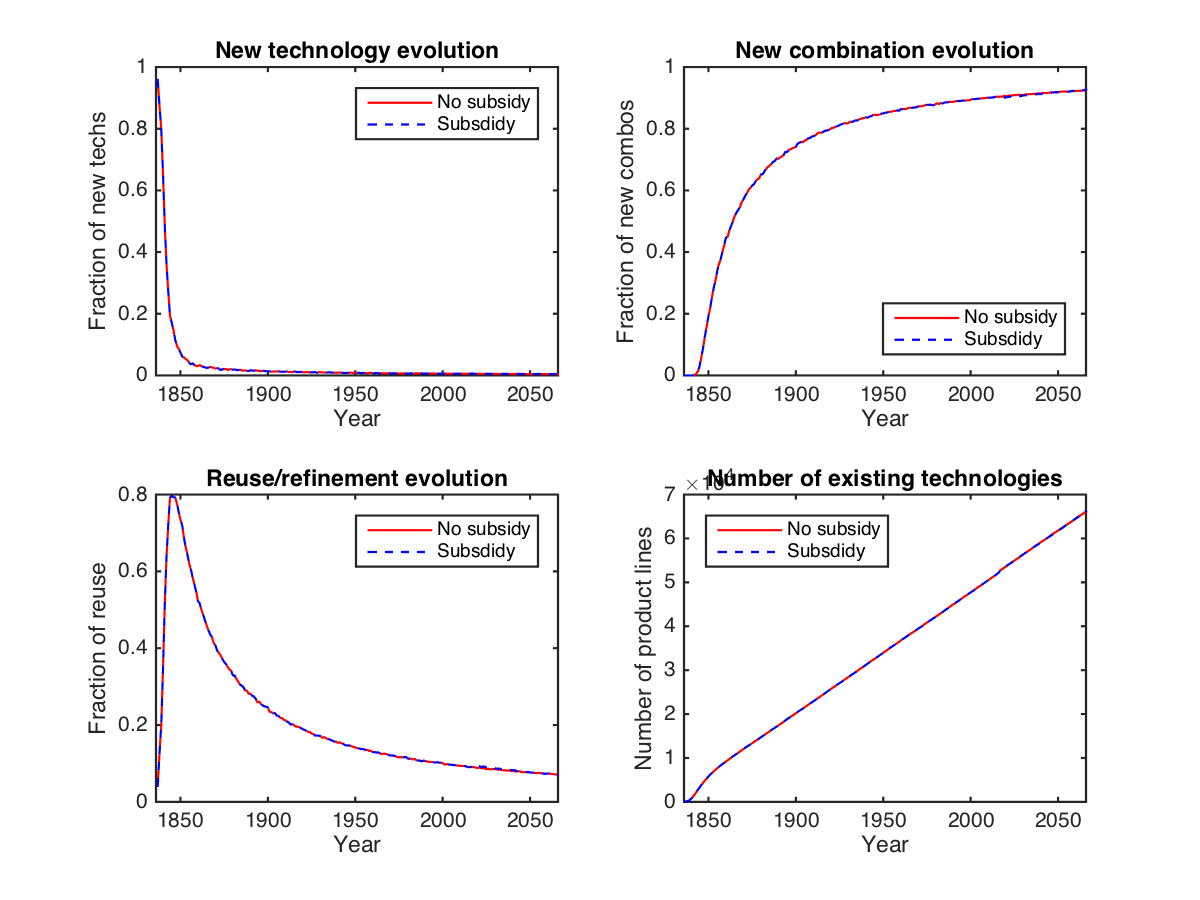
\includegraphics[scale=.6]{patentsNC_50y}
\caption{Evolution of patent shares across the whole period}
\end{figure}

\begin{figure}
\centering
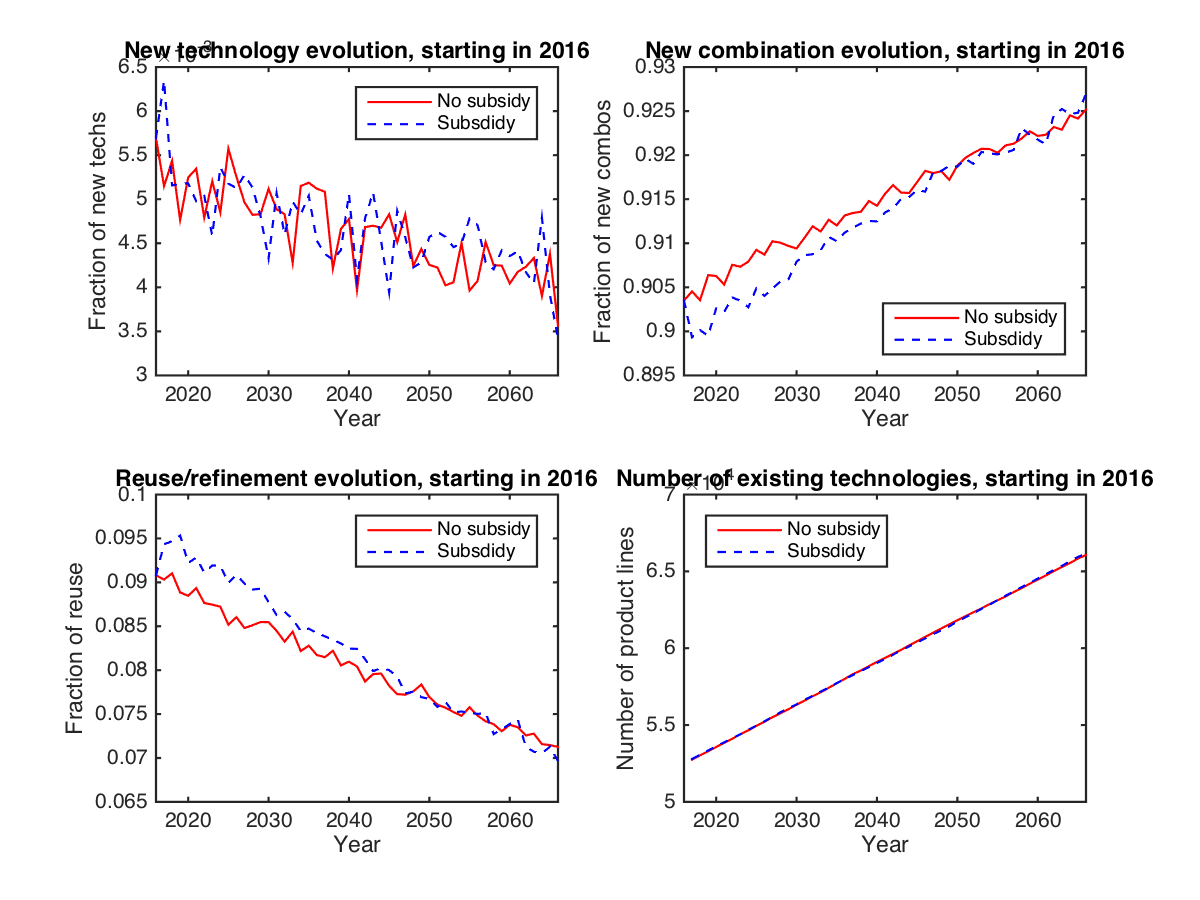
\includegraphics[scale=.6]{patents2016NC_50y}
\caption{Evolution of patent shares, starting in 2016}
\end{figure}

\begin{figure}
\centering
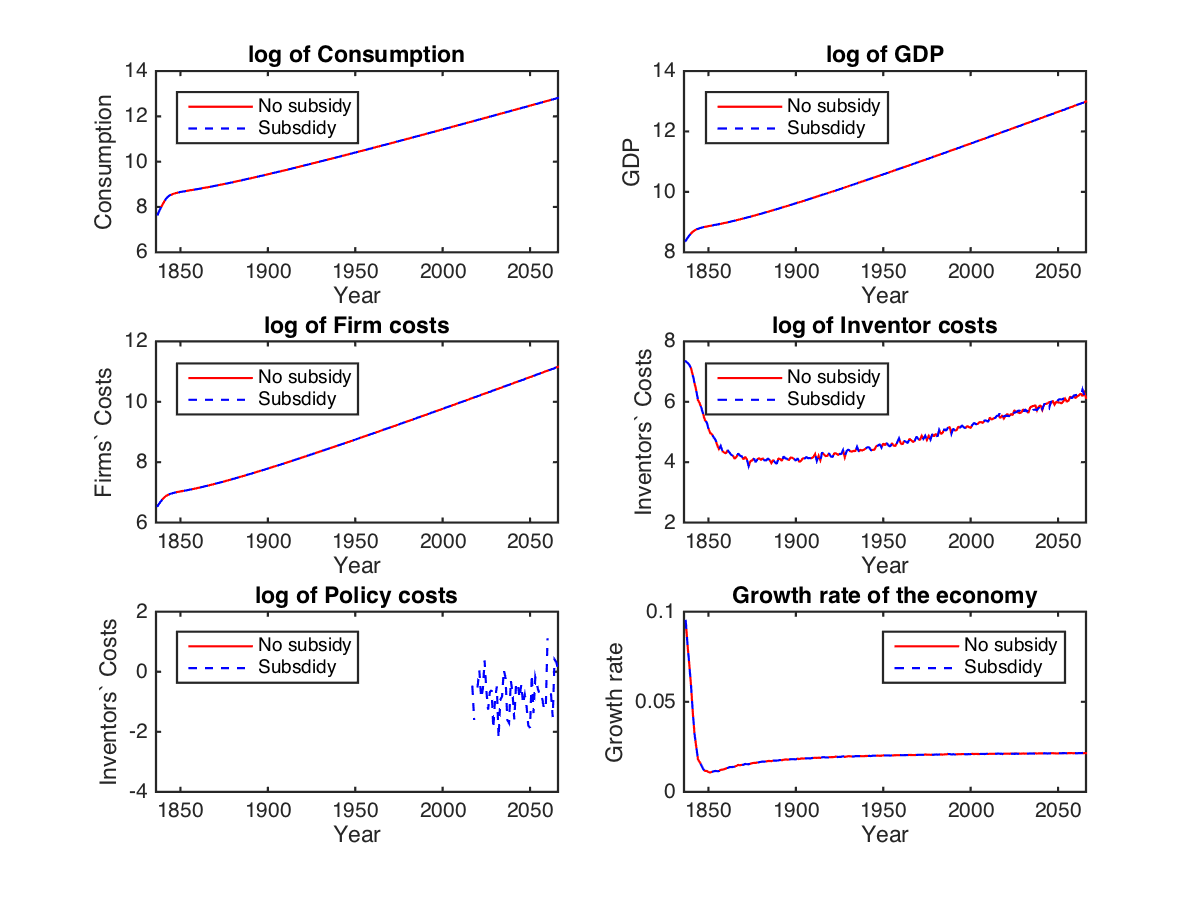
\includegraphics[scale=.6]{aggregatesNC_50y}
\caption{Evolution of aggregate variables over the whole period}
\end{figure}

\begin{figure}
\centering
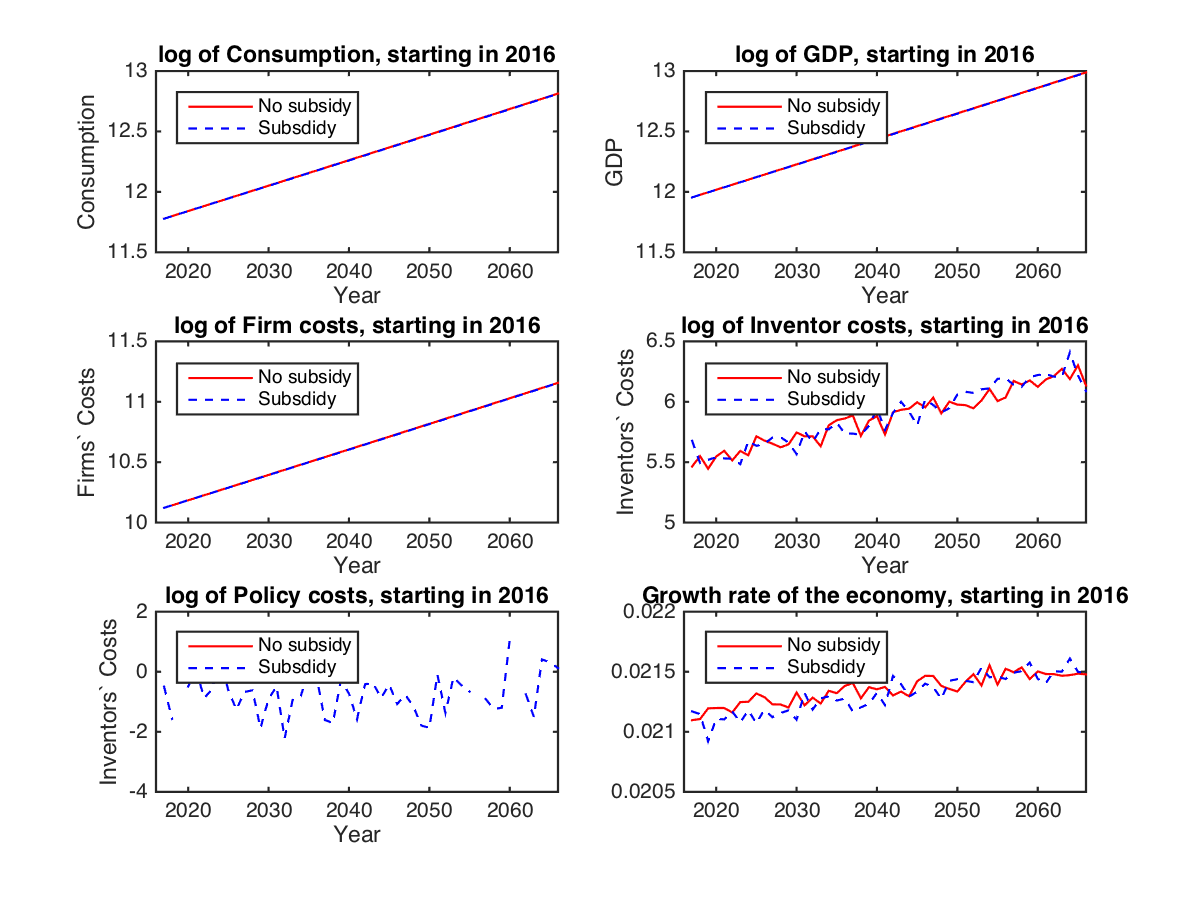
\includegraphics[scale=.6]{aggregates2016NC_50y}
\caption{Evolution of aggregate variables starting in 2016}
\end{figure}

\begin{figure}
\centering
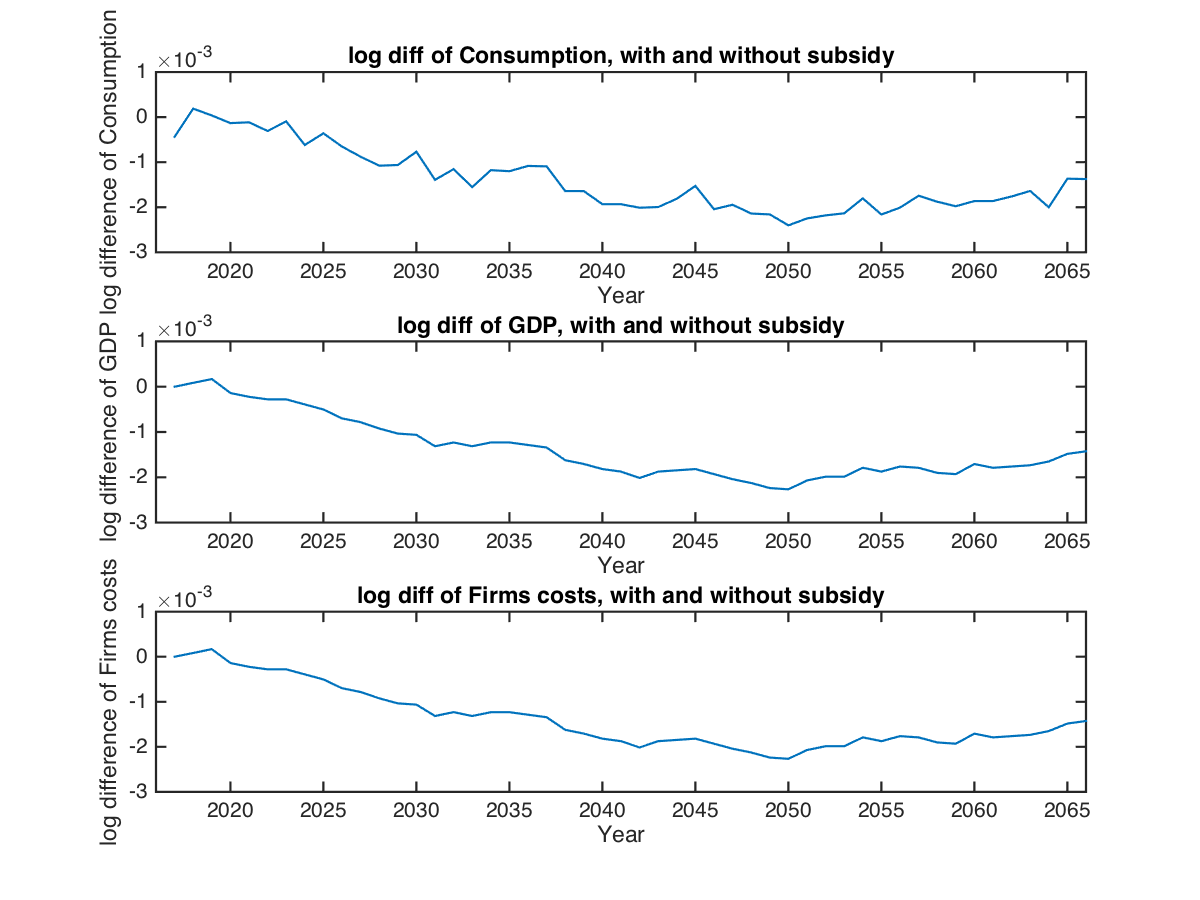
\includegraphics[scale=.6]{aggregates_diffNC_50y}
\caption{Log difference of variables, with subsidy - without subsidy, starting in 2016.}
\end{figure}

\begin{figure}
\centering
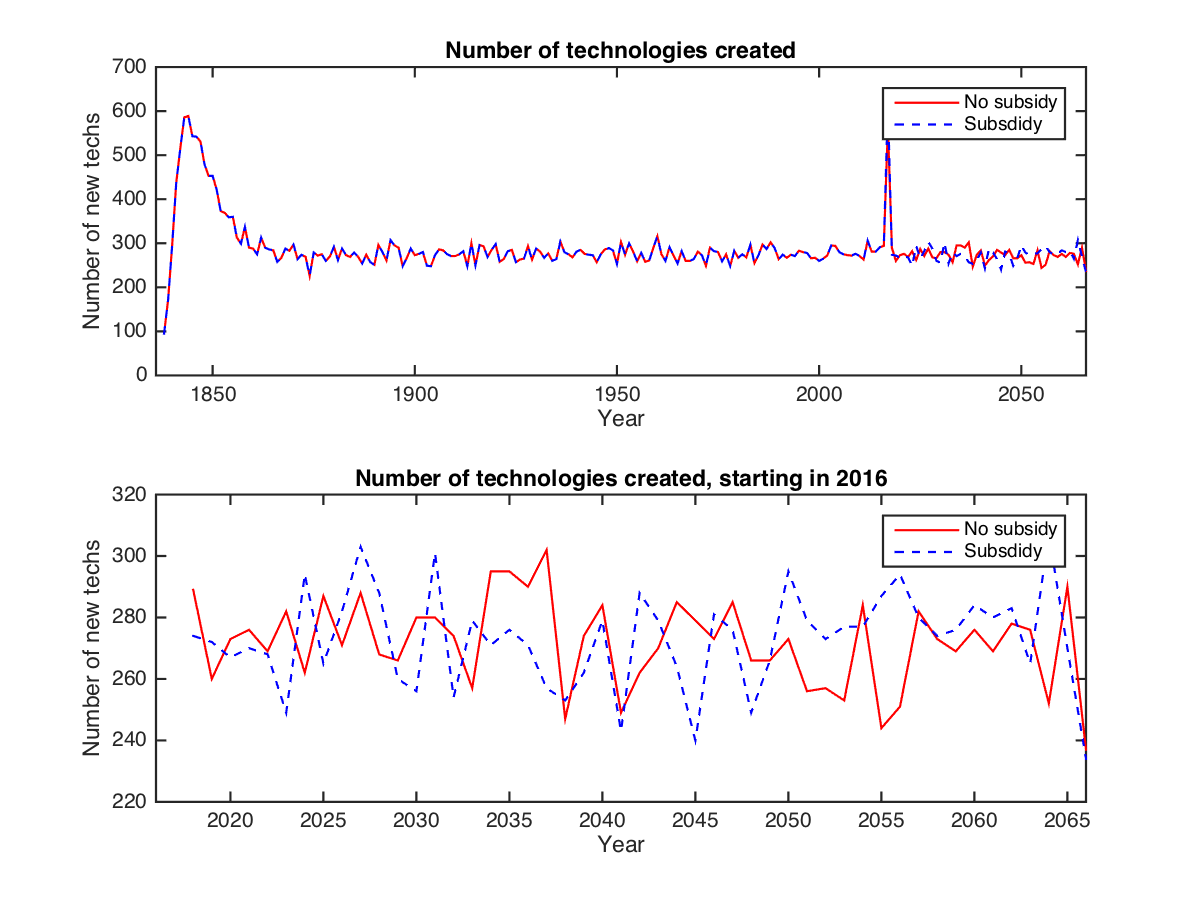
\includegraphics[scale=.6]{tech_creationNC_50y}
\caption{Number of technologies created every year (Ignore the spike around 2020).}
\end{figure}








\end{document}
